%!TEX root = main.tex

%\subsection{Android multitasking mechanism}

In this section, we briefly review the core concepts regarding the android multitasking mechanism, i.e., activities and fragments, and the evolution of the back stack. 
 
\subsection{Activity, task and task stack}
For the purpose of this paper, an Android app can be considered as a collection of \emph{activities}. At any time, there is one activity displayed on the screen of the device. 
The activities are organized into tasks. 
A \emph{task} is a collection of activities %that users interact with when performing 
to carry out a certain job. The running activities within a task are managed as an \emph{activity stack} 
%\emph{back stack} % this has been changed on 14/11/21
following the order that an activity is opened. In the activity stack, there are two distinguished activities, i.e., the \emph{root activity} and \emph{top activity}, which are sitting at the bottom and top of the stack respectively. %Note that %the back stack evolves in a way that the role of apps is diminished, in the  sense that
%in Android, activities from different apps can stay in the same task, and activities from the same app can enter different tasks.

The Android system normally run multiple tasks which are organized as the \emph{task stack}. The top task is the \emph{foreground} task whiles others are \emph{background} tasks. %They are organized as a task stack.
% as well, which is %for managing the current foreground task and previous background tasks. 
%referred to as a \emph{task stack} \cite{LHR17} (aka. activity stack \cite{RZXWL15}). 
%where The foreground task, as expected, sits on the top of the task stack. 
%
When a task comes to the foreground, its top activity is displayed on the device screen. When an activity finishes, it is popped from the activity stack. If the activity stack is not empty, the new top activity is displayed on the screen. Otherwise, the task itself finishes in which case it is popped from the task stack.  
We mention that, the Home screen comes to the foreground when a user presses the Home button (in this case the task stack will be emptied) or when the task stack becomes empty. The task stack  is the central data structure for Android multi-tasking mechanism, and we are mostly interested in its evolution in response to activity activation. When an activity is started, there are three basic attributes which determine the resulting task stack: \emph{launch modes, task affinities}, and \emph{intent flags}. %Developers can specify how to activate target activities
%The task stack is the central data structure for the Android multi-tasking mechanism, and we are mostly interested in its evolution in response to activity activation. 

 All the activities of an app, as well as their launch modes and task affinities, are defined in the \emph{manifest file}  
 ({\sf AndroidManifest.xml}). Differently, intent flags are set by caller activities to declare how to activate target activities by calling startActivity() or startActivityForResult() with the intent flags as its arguments. The launch mode attribute  specifies one of four modes to launch an activity: standard, singleTop, singleTask, and singleInstance, with standard being the default. A standard or singleTop activity can be instantiated multiple times leading to duplicated activities in a task. In contrast, an activity with the singleTask or singleInstance launch mode should be instantiated only once. Furthermore, an activity with the singleInstance launch mode is always the root activity of a task. While a singleTask activity
 can contain other standard or singleTop activities in its task, a singleInstance activity does not contain any other
 activities in its task. It is the only activity in its task; if it starts another activity, that activity is assigned to a different task. 
The task affinity attribute is of string data type and specifies to which task the activity prefers to belong. By default, all the activities from the same app have the same affinity, the package name of the app (i.e., all activities in the same app prefer to be in the same task). However, one can modify the default affinity of the activity. Android allows a great degree of flexibility: activities defined in different apps can share a task affinity whilst activities defined in the same app can be assigned with different task affinities.  

 
Android supports inter-component communication via \emph{intents}. An intent is an asynchronous message that activates activities. 
Android provides two types of intents, \emph{explicit} intents and \emph{implicit} intents. 
Explicit intents specify directly which activity to activate. Implicit intents, on the other hand, do not directly specify the activities which should be called, it only specifies actions to be performed. 
%A Uri can be used with the implicit intent to specify the data type.
For example, an implicit intent with the action ``ACTION\_VIEW'' and the data of the URI ``http://www.google.com'' will cause a web browser to open a webpage. 
Android system searches for all activities which are registered for the specific action and the data type. If many activities are found then the user can select which activities to use.
In this paper, we restrict our attention to explicit intents since our focus is to understand the evolvement of the back stack when activities are started, and we do not attack the (another challenging) problem of resolving which activity should be started by implicit intents. 

Android provides 23 intent flags related to activities (see \cite{intentflags} for the detailed description of the intent flags). Intent flags are set by caller activities to declare how to activate target activities and are passed to startActivity() or startActivityForResult() as their arguments. 
%A detailed description of the meanings of these intent flags can be found in \url{https://developer.android.com/reference/android/content/Intent#flags}.
In this paper, among the 23 intent flags, we consider the following 10 ones, 
\begin{itemize}
	\item $\rm FLAG\_ACTIVITY\_NEW\_TASK$,
	\item $\rm FLAG\_ACTIVITY\_NEW\_DOCUMENT$,
	\item $\rm FLAG\_ACTIVITY\_MULTIPLE\_TASK$,
	\item $\rm FLAG\_ACTIVITY\_SINGLE\_TOP$,
	\item $\rm FLAG\_ACTIVITY\_REORDER\_TO\_FRONT$,
	\item $\rm FLAG\_ACTIVITY\_CLEAR\_TOP$,
	\item $\rm FLAG\_ACTIVITY\_CLEAR\_TASK$,
	\item $\rm FLAG\_ACTIVITY\_PREVIOUS\_IS\_TOP$,
	\item $\rm FLAG\_ACTIVITY\_NO\_HISTORY$,
	\item $\rm FLAG\_ACTIVITY\_TASK\_ON\_HOME$.
	%\item $FLAG\_ACTIVITY\_EXCLUDE\_FROM\_RECENTS$ (FAEFR),
	%	\item $\dots$.
\end{itemize}
\hide{
\begin{itemize}
	\item $\rm FLAG\_ACTIVITY\_NEW\_TASK$: this flag is set when the user wants to create a new task when starting an activity, 
	\item $\rm FLAG\_ACTIVITY\_NEW\_DOCUMENT$: this flag is set so that each instance of the activity (hosting a document) is put in a new task,
	\item $\rm FLAG\_ACTIVITY\_MULTIPLE\_TASK$: this flag is used to create a new task and launch an activity into it,
	\item $\rm FLAG\_ACTIVITY\_SINGLE\_TOP$: this flag is set so that the activity will not be launched if it is already running at the top of the history stack,
	\item $\rm FLAG\_ACTIVITY\_REORDER\_TO\_FRONT$: this flag will cause the launched activity to be brought to the front of its task if it is already running,
	\item $\rm FLAG\_ACTIVITY\_CLEAR\_TOP$: if this flag is set, then when the activity being launched is already running in the current task, instead of launching a new instance of that activity, all of the other activities on top of it will be closed,
	\item $\rm FLAG\_ACTIVITY\_CLEAR\_TASK$: if this flag is set, then any existing task that would be associated with the activity will be cleared before the activity is started,
	\item $\rm FLAG\_ACTIVITY\_PREVIOUS\_IS\_TOP$: if this flag is set, then the activity immediately below the foreground activity in the topmost task will be taken as the top activity for deciding whether a new instance of this activity should be created,
	\item $\rm FLAG\_ACTIVITY\_NO\_HISTORY$: if set, then the activity will be launched but not stored into the task stack, 
	\item $\rm FLAG\_ACTIVITY\_TASK\_ON\_HOME$: if this flag is set, then all the tasks, except the current home activity task, will be removed, and a new task is created to host this activity and pushed on top of the home activity task.
	%\item $FLAG\_ACTIVITY\_EXCLUDE\_FROM\_RECENTS$ (FAEFR),
	%	\item $\dots$.
\end{itemize}
}
The other 13 intent flags are ignored, for various reasons as shown in Table~\ref{tab-int-flag-ignore}.
\begin{table}[htbp]
\begin{center}
\small
    \begin{tabular}{|m{5.5cm}<{\centering}|m{8.5cm}<{\centering}|}
    \hline
    \textbf{Intent Flags} & \textbf{Reasons for being ignored in this paper}  \\
    \hline
	$\rm FLAG\_ACTIVITY\_REQUIRE\_DEFAULT$ & \multirow{3}*{Related to implicit intents, which we do not consider in this paper.}\\
	\cline{1-1}
	$\rm FLAG\_ACTIVITY\_REQUIRE\_NON\_BROWSER$ &\\
	\cline{1-1}
	$\rm FLAG\_ACTIVITY\_MATCH\_EXTERNAL$ & \\
    \hline
	$\rm FLAG\_ACTIVITY\_FORWARD\_RESULT$ & Used for transferring results between activities, which we do not consider in this paper.\\
    \hline
	$\rm FLAG\_ACTIVITY\_RETAIN\_IN\_RECENTS$  & \multirow{2}*{\shortstack{Related to the recent app list, which we do not consider it in this paper.}}\\
	\cline{1-1}
	$\rm FLAG\_ACTIVITY\_EXCLUDE\_FROM\_RECENTS$ &\\
    \hline
	$\rm FLAG\_ACTIVITY\_CLEAR\_WHEN\_TASK\_RESET$ & Deprecated from Android 5.0.\\
    \hline
	$\rm FLAG\_ACTIVITY\_BROUGHT\_TO\_FRONT$ & \multirow{2}*{Can only be set by Android operating system, not set by application code.}\\
	\cline{1-1}
	$\rm FLAG\_ACTIVITY\_LAUNCHED\_FROM\_HISTORY$ &\\
    \hline
	$\rm FLAG\_ACTIVITY\_NO\_USER\_ACTION$ & Related to the life-cycle of activities and we do not model the life-cycle of activities in this paper.\\
    \hline
	$\rm FLAG\_ACTIVITY\_NO\_ANIMATION$ &Used to show some animation when starting an activity and is not related to the evolvement of the back stack.\\
    \hline
	$\rm FLAG\_ACTIVITY\_LAUNCH\_ADJACENT$ & Related to the split-screen mode, which we do not consider in this paper.\\
    \hline
	$\rm FLAG\_ACTIVITY\_RESET\_TASK\_IF\_NEEDED$ & Related to the ``allowTaskReparenting'' attribute of activities, which we do not consider in this paper.\\
    \hline
    \end{tabular}
\end{center}
    \caption{Reasons for ignoring some intent flags in this paper}
    \label{tab-int-flag-ignore}
\end{table}

Besides launch modes, task affinities, and intent flags, there are some other factors that may also affect the behaviors of the task stack. 
When a caller activity calls startActivity() or startActivityForResult() to start a callee activity, the caller activity can also call the \emph{finish()} procedure so that when the callee activity is started, the caller activity is finished. 
Moreover, the \emph{real activity}\footnote{The name is inherited from the Android system.} of a task also matters. The real activity of a task is the activity that was pushed into the task as the bottom activity when the task was created. 
%Intuitively, $A_i$ is the activity which was pushed into the task---as the bottom activity---when the task $S_i$ was created. (Note that $A_i$ is not necessarily the current bottom activity of $S_i$.) 
If the real activity of a task is $B$ and the task is not the main task, then attempting to push an instance of $B$ to the task will not modify the task. 



\hide{
\begin{itemize}
\item The following three flags are related to implicit intents, which we do not consider in this paper:\\
 $\rm FLAG\_ACTIVITY\_REQUIRE\_DEFAULT$, $\rm FLAG\_ACTIVITY\_REQUIRE\_NON\_BROWSER$, \\
 $\rm FLAG\_ACTIVITY\_MATCH\_EXTERNAL$. 

\item The flag $\rm FLAG\_ACTIVITY\_FORWARD\_RESULT$ is for transferring results between activities, since we ignore results transferred between activities.

\item The two flags $\rm FLAG\_ACTIVITY\_RETAIN\_IN\_RECENTS$ and $\rm FLAG\_ACTIVITY\_EXCLUDE\_FROM\_RECENTS$ are ignored, since the recent app list is a data structure independent of the back stack and we do not consider it in this paper. 

\item The flag $\rm FLAG\_ACTIVITY\_CLEAR\_WHEN\_TASK\_RESET$ is deprecated from Android 5.0, thus ignored. 

\item The flags $\rm FLAG\_ACTIVITY\_BROUGHT\_TO\_FRONT$ and $\rm FLAG\_ACTIVITY\_LAUNCHED\_FROM\_HISTORY$ are ignored, since they can only be set by Android operating system, not set by application code. 

\item The flag $\rm FLAG\_ACTIVITY\_NO\_USER\_ACTION$ is related to the life-cycle of activities and we do not model the life-cycle of activities in this paper, thus ignored. 

\item The flag $\rm FLAG\_ACTIVITY\_NO\_ANIMATION$ is used to show some animation when starting an activity and is not related to the evolvement of the back stack, thus ignored. 

\item The flag $\rm FLAG\_ACTIVITY\_LAUNCH\_ADJACENT$ is related to the split-screen mode and we do not consider split-screen in this paper, thus ignored.  
%
\item The flag $\rm FLAG\_ACTIVITY\_RESET\_TASK\_IF\_NEEDED$ is related to the ``allowTaskReparenting'' attribute of activities, which we do not consider in this paper, thus this flag is ignored.  
\end{itemize}
}

 %%%%%%%%%%%%%%texts removed%%%%%%%%%%%%%%
 %%%%%%%%%%%%%%texts removed%%%%%%%%%%%%%%
  %%%%%%%%%%%%%%texts removed%%%%%%%%%%%%%%
 \hide{
 \revision{Among these 23 intent flags, we consider the following eleven, namely,}
\begin{itemize}
	\item $\rm FLAG\_ACTIVITY\_NEW\_TASK$ ($\ntkflag$),
	\item $\rm FLAG\_ACTIVITY\_NEW\_DOCUMENT$ ($\ndmflag$),
	\item $\rm FLAG\_ACTIVITY\_MULTIPLE\_TASK$ ($\mtkflag$),
	\item $\rm FLAG\_ACTIVITY\_SINGLE\_TOP$ ($\stpflag$),
	\item $\rm FLAG\_ACTIVITY\_REORDER\_TO\_FRONT$ ($\rtfflag$),
	\item $\rm FLAG\_ACTIVITY\_CLEAR\_TOP$ ($\ctpflag$),
	\item $\rm FLAG\_ACTIVITY\_CLEAR\_TASK$ ($\ctkflag$),
	\item $\rm FLAG\_ACTIVITY\_PREVIOUS\_IS\_TOP$ ($\pitflag$),
	\item $\rm FLAG\_ACTIVITY\_NO\_HISTORY$ ($\nohflag$),
	\item $\rm FLAG\_ACTIVITY\_RESET\_TASK\_IF\_NEEDED$ ($\rtnflag$),
	\item $\rm FLAG\_ACTIVITY\_TASK\_ON\_HOME$ ($\tohflag$).	
	%\item $FLAG\_ACTIVITY\_EXCLUDE\_FROM\_RECENTS$ (FAEFR),
	%	\item $\dots$.
\end{itemize}

\revision{The exclusion of the remaining 12 intent flags is justified as follows:}
\begin{itemize}
    \item $\rm FLAG\_ACTIVITY\_BROUGHT\_TO\_FRONT$: This flag is not normally set by application code, but set by system.
    \item $\rm FLAG\_ACTIVITY\_LAUNCHED\_FROM\_HISTORY$: This flag is not normally set by application code, but set by system.
%
    \item $\rm FLAG\_ACTIVITY\_CLEAR\_WHEN\_TASK\_RESET$: This flag was deprecated in API level 21 (Android 5.0).
%
    \item $\rm FLAG\_ACTIVITY\_LAUNCH\_ADJACENT$: This flag is only used for split-screen multi-window mode. The split screen is ignored at present, thus ignored.
%
    \item $\rm FLAG\_ACTIVITY\_RETAIN\_IN\_RECENTS$: If set, the new activity will remain in the recent task when it is finished. Recent task is different from back stack and not modeled, thus ignored.
%
    \item $\rm FLAG\_ACTIVITY\_EXCLUDE\_FROM\_RECENTS$: If set, the new activity is not kept in the recent task. Recent task is different from back stack and not modeled, thus ignored.
%
    \item $\rm FLAG\_ACTIVITY\_REQUIRE\_NON\_BROWSER$: If set, this flag will only launch the intent if it resolves to a result that is not a browser. If no such result exists, an ActivityNotFoundException will be thrown. In principle, we can support it if we know which activities belong to browsers. The current model extraction tool does not obtain such info, thus ignored.
%
    \item $\rm FLAG\_ACTIVITY\_REQUIRE\_DEFAULT$: If set, this flag will only launch the intent if it resolves to a single result. If no such result exists or if the system chooser would otherwise be displayed, an ActivityNotFoundException will be thrown. The implicit intent is not considered at present, thus ignored.
%
    \item $\rm FLAG\_ACTIVITY\_NO\_USER\_ACTION$: If set, this flag will prevent the normal Activity.onUserLeaveHint() callback from occurring on the current frontmost activity before it is paused as the newly-started activity is brought to the front. The lifecycle is not modeled at present, thus ignored.
%
    \item $\rm FLAG\_ACTIVITY\_NO\_ANIMATION$: If set, this flag will prevent the system from applying an activity transition animation to go to the next activity. The animation is ignored, since it does not affect back stack.
%
    \item $\rm FLAG\_ACTIVITY\_MATCH\_EXTERNAL$: If set, this flag will attempt to launch an instant app if no full app on the device can already handle the intent. It does not affect back stack thus ignored.
%
    \item $\rm FLAG\_ACTIVITY\_FORWARD\_RESULT$: If set, this flag is being used to launch a new activity from an existing one, then the reply target of the existing activity will be transferred to the new activity. This way, the new activity can call Activity.setResult(int) and have that result sent back to the reply target of the original activity. The result transfer between activities is ignored at present, thus ignored.
\end{itemize}
}
 %%%%%%%%%%%%%%texts removed%%%%%%%%%%%%%%
 %%%%%%%%%%%%%%texts removed%%%%%%%%%%%%%%
  %%%%%%%%%%%%%%texts removed%%%%%%%%%%%%%%

%When an activity is started, there are three basic attributes which determine the resulting task stack: \emph{launch mode, task affinity}, and \emph{intent flags}. Their underpinning machinery is relatively well-understood and has been %studied and 
%captured in the previous formalisations \cite{LHR17,ChenHSWWY18,HCWWY19}, and are also fully incorporated in the current modeling.  %Developers can specify how to activate target activities
%

%All the activities of an app, as well as their launch modes and task affinities, are defined in the \emph{manifest file}  
%({\sf AndroidManifest.xml}). Differently, intent flags are set by caller activities to declare how to activate target activities by calling startActivity() or startActivityForResult() with the intent flags as its arguments. The launch mode attribute   specifies one of four modes to launch an activity: standard, singleTop, singleTask, and singleInstance, with standard being the default. 


% Android system will find the target task in the task stack for the caller activity by calling getOrCreateRootTask() in line 2833 in the RootWindowContainer.java file first, and then place the caller activity in the target task by calling complyActivityFlags() in line 2411 in the ActivityStarter.java file. In the first step, Android system will search for a task whose real activity matches the caller activity first. If there is no such task found, then it will search for a task whose task affinity matches the the task affinity of the caller activity. If there is no such task found, then it will create a task for the caller activity. In the second step, Android system will place the activity in the target according to the launch mode of the caller activity and the intent flags.
% \begin{figure}[htbp]
%         \centering
%         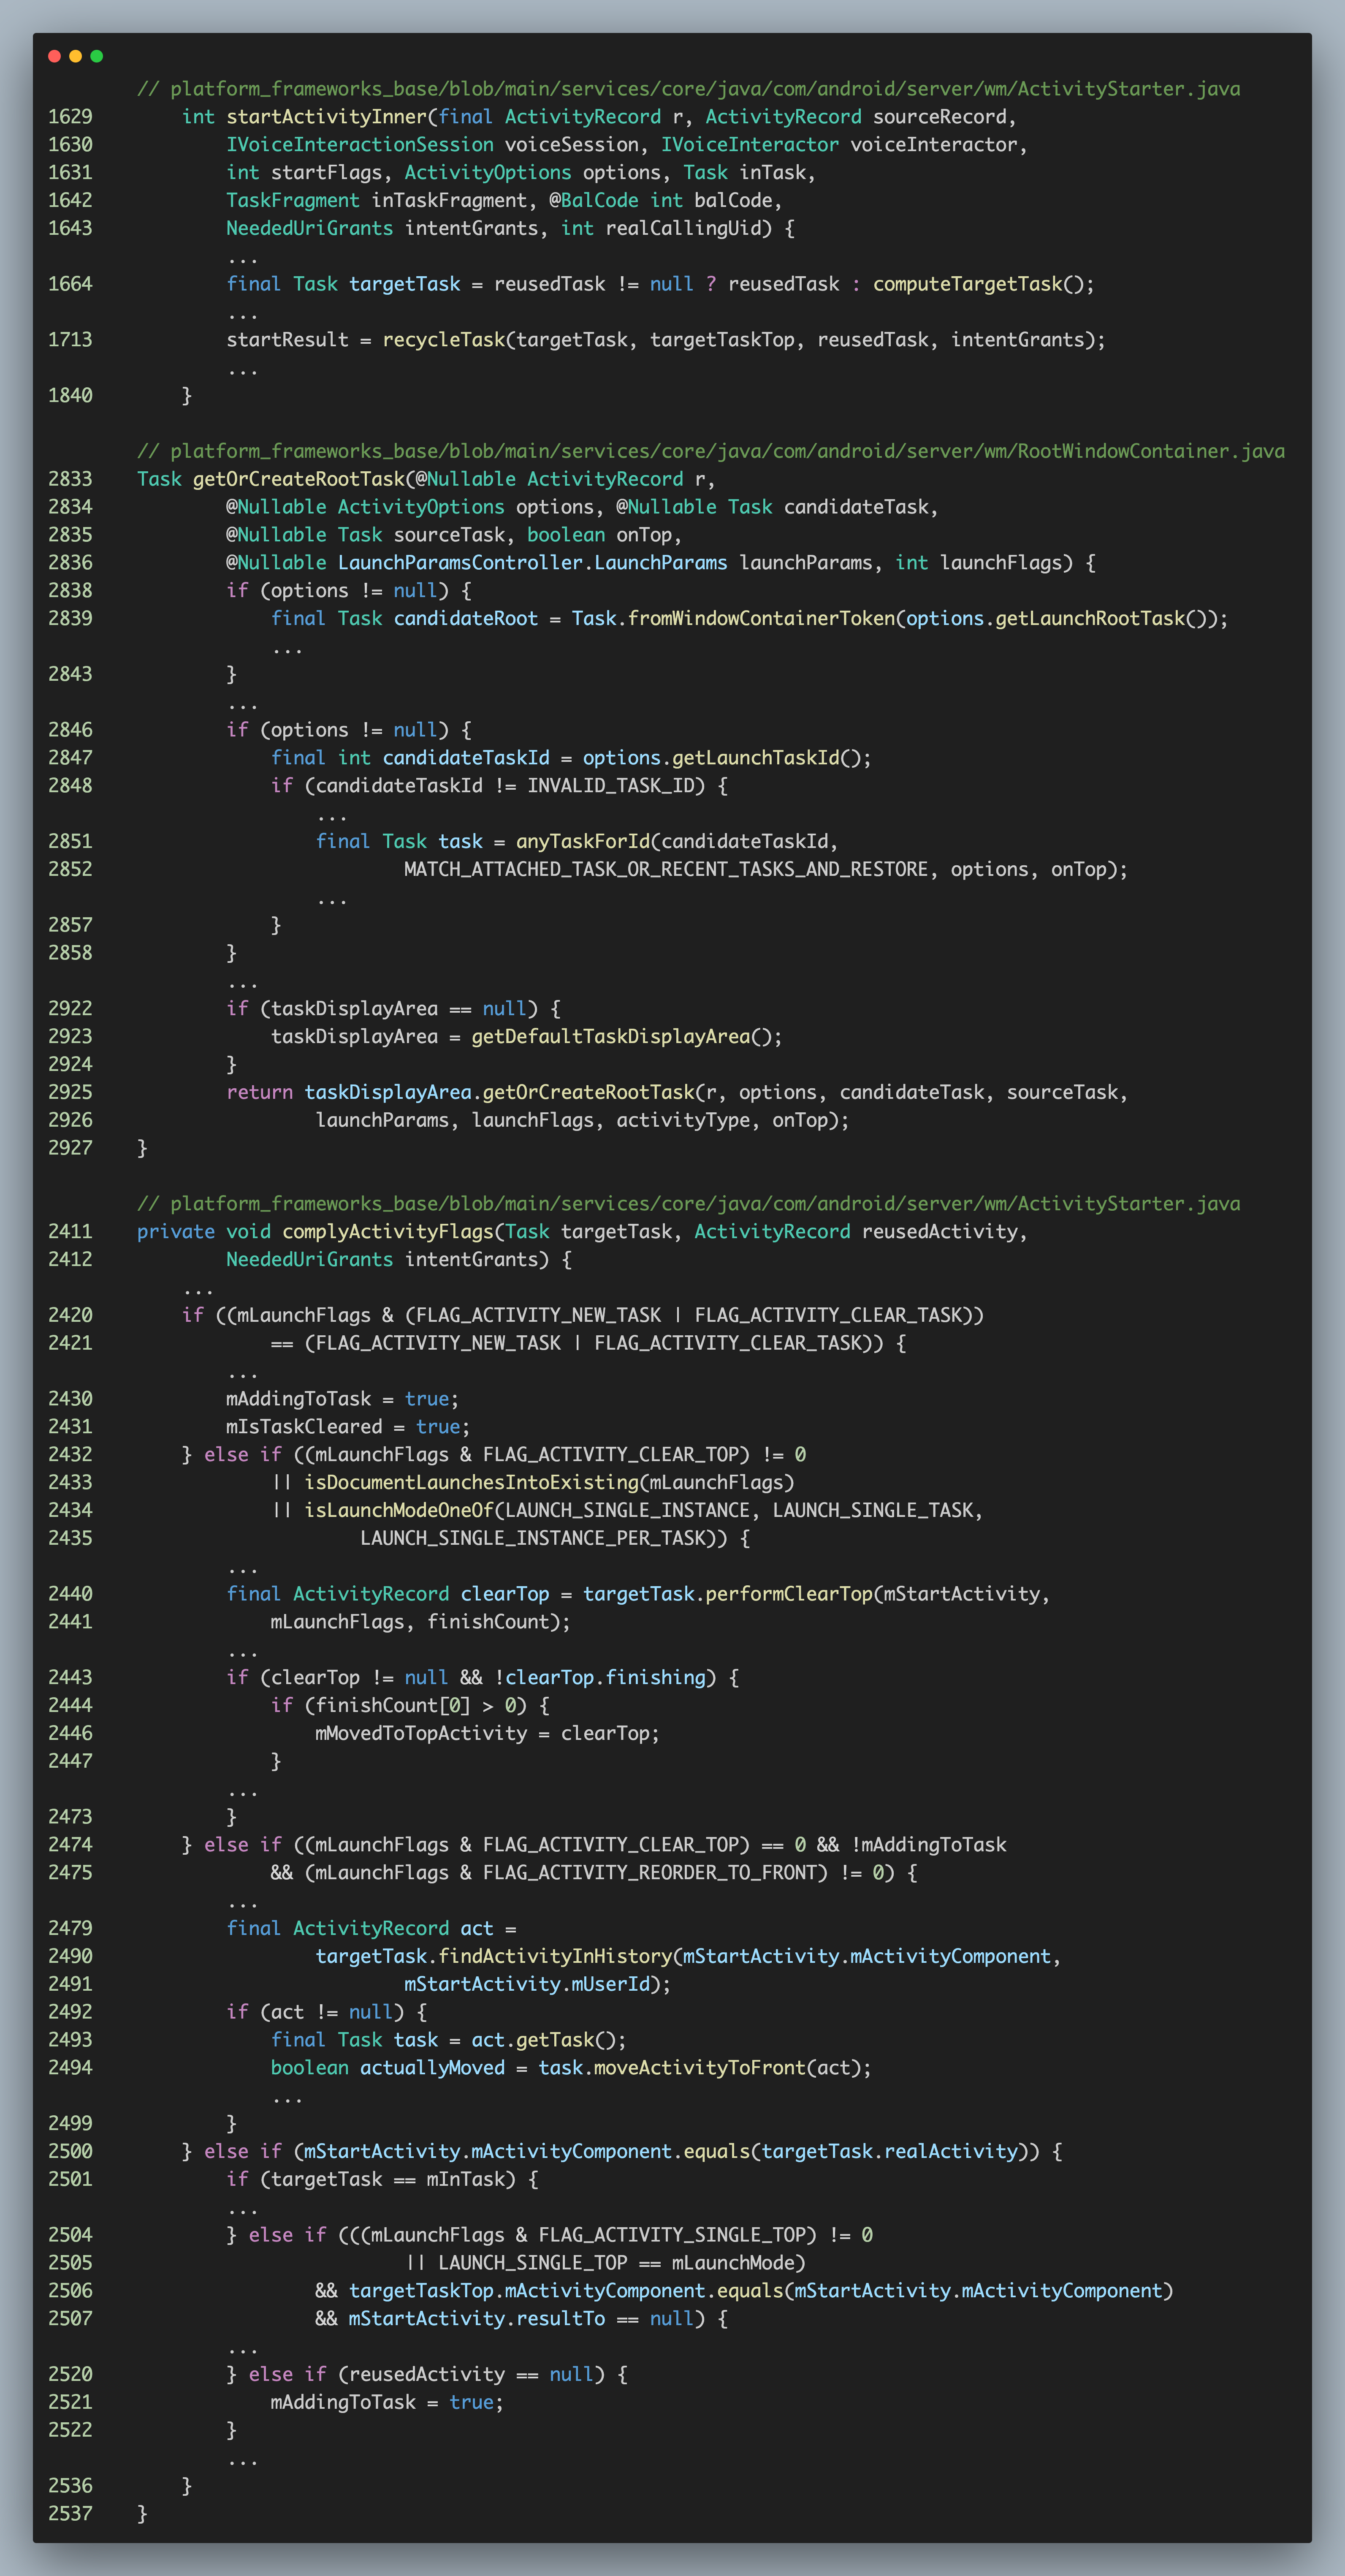
\includegraphics[scale = 0.08]{activity-code.png}
%         \caption{Android system source code for starting activity.}
%     \label{activity-code}
% \end{figure}
% \smallskip

% \begin{figure}[htbp]
%         \centering
%         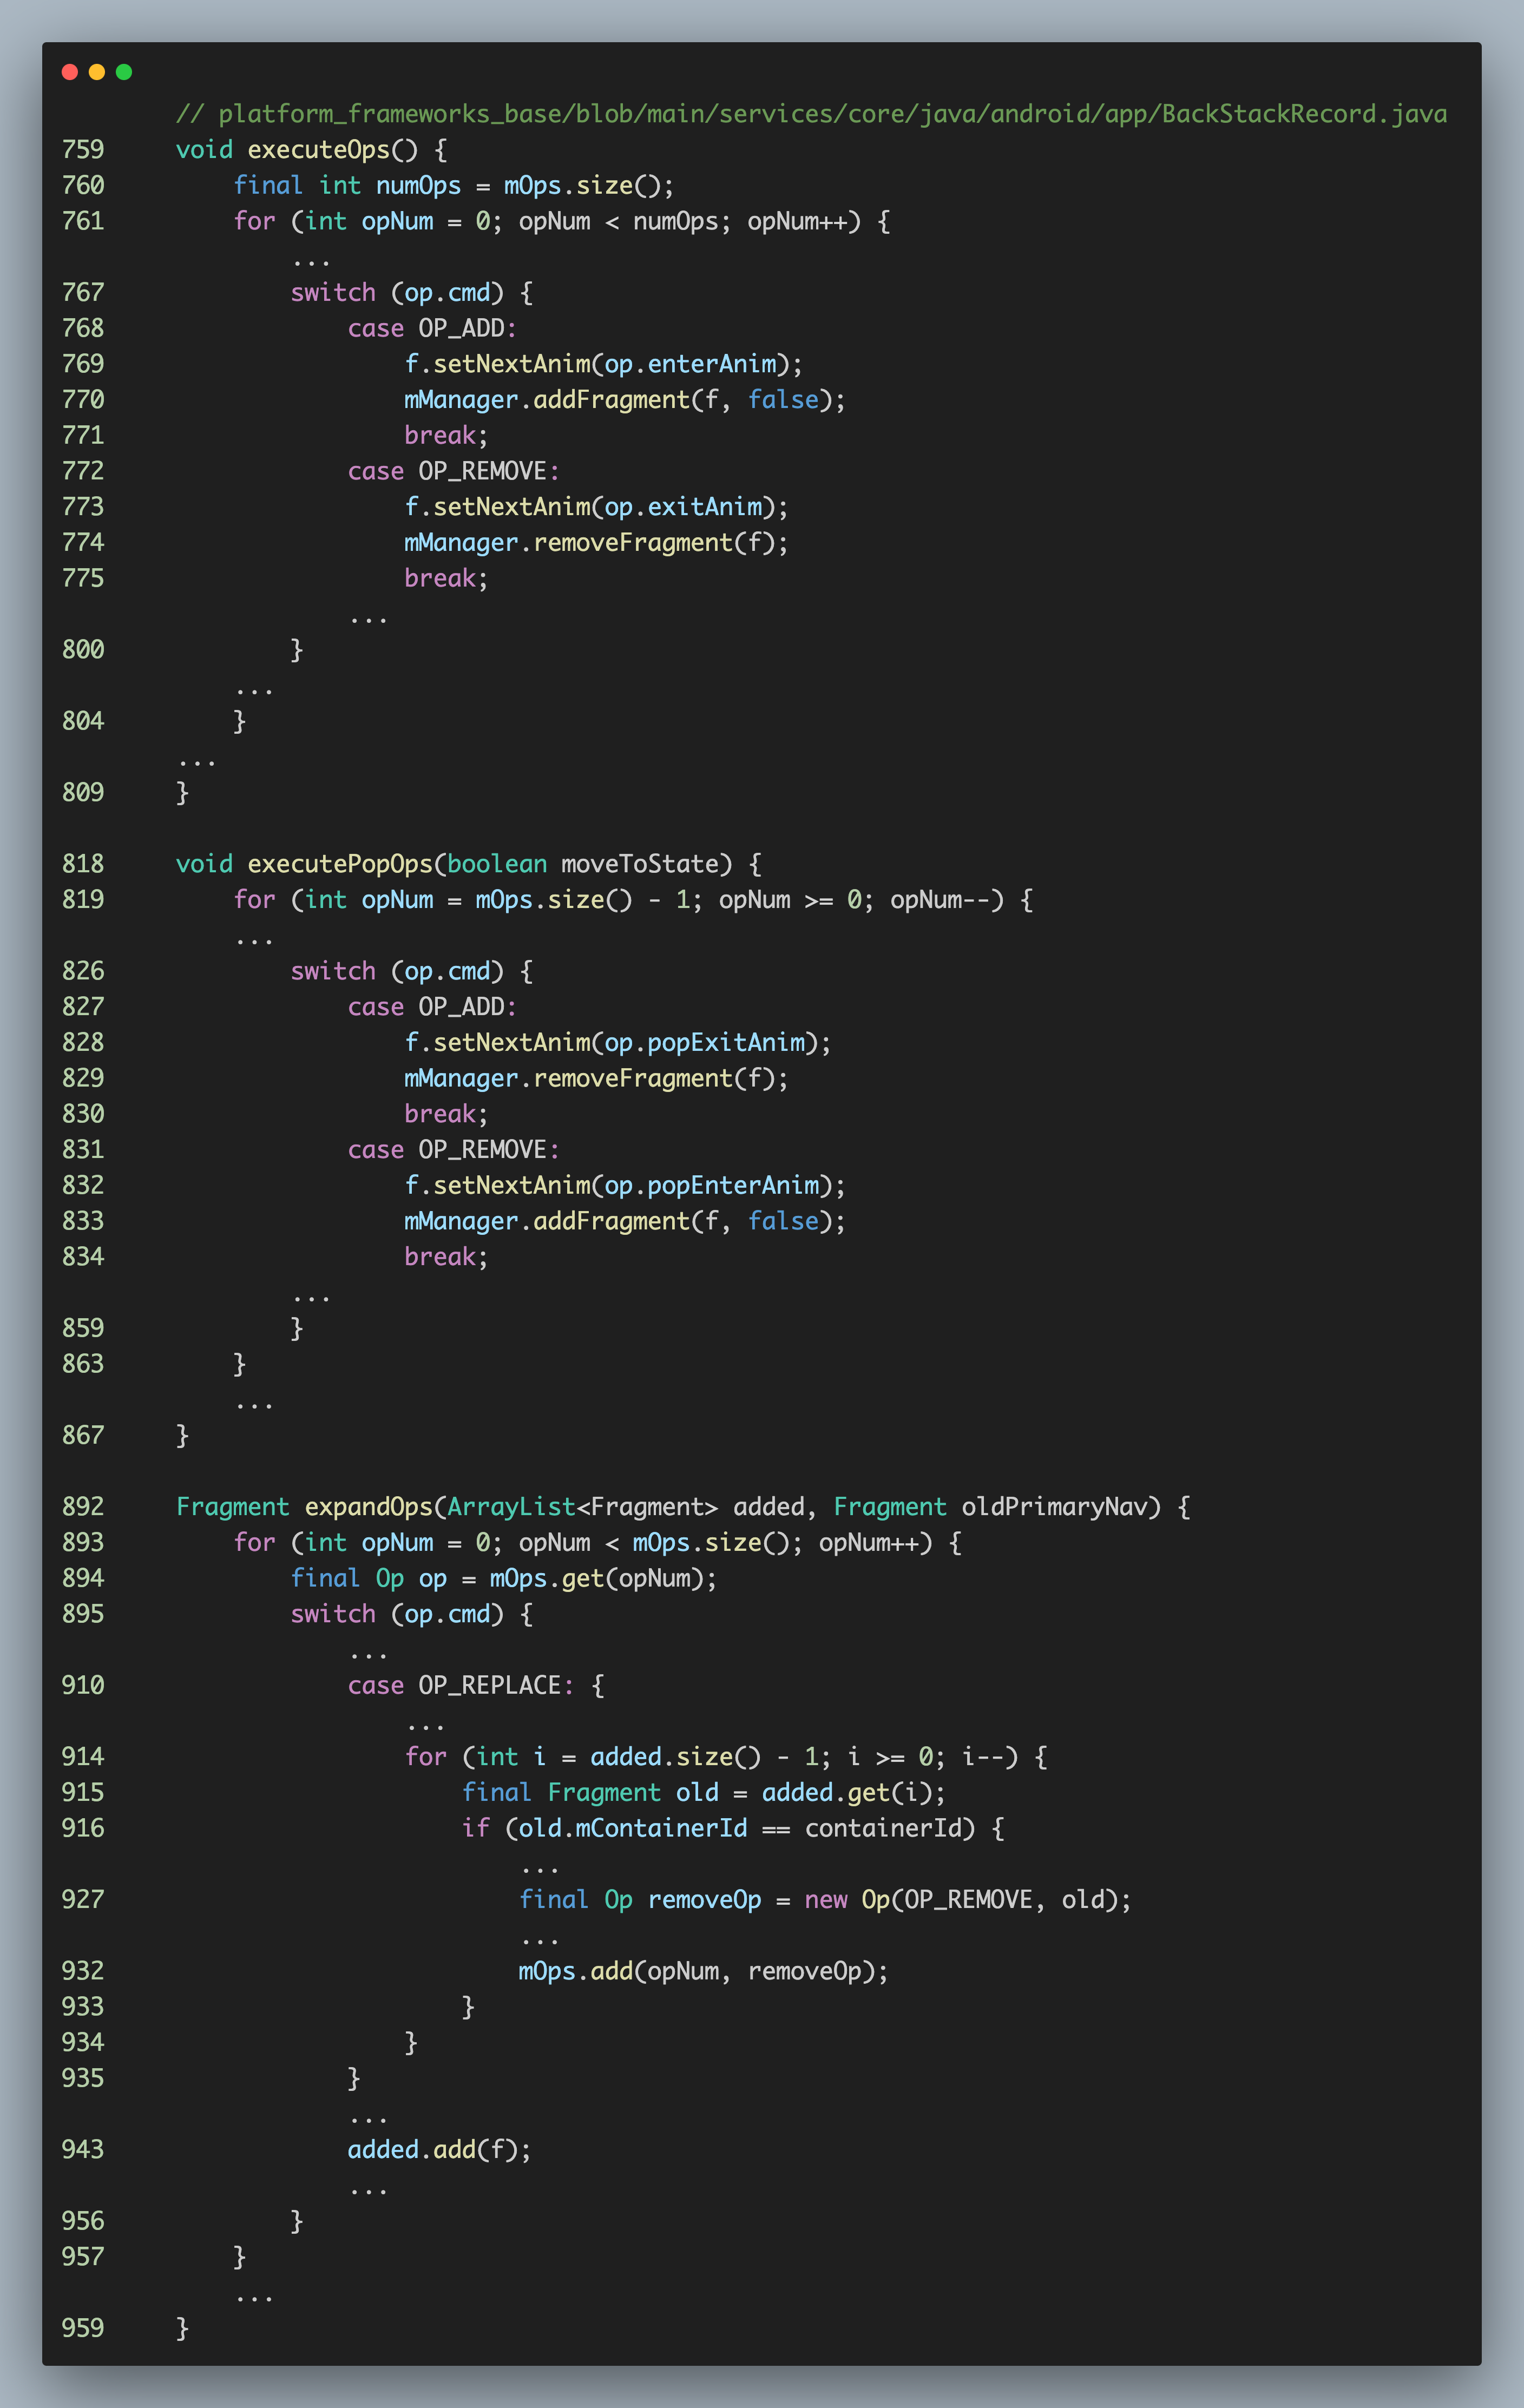
\includegraphics[scale = 0.09]{fragment-code.png}
%         \caption{Android system source code for starting fragment.}
%     \label{fragment-code}
% \end{figure}
% \smallskip


\subsection{Fragment, fragment stack, fragment transaction and fragment transaction stack}

Importantly, activities are \emph{not} an atomic object and may contain sub-components such as %view groups and 
fragments. %which are one of the main focuses here. 
Previous formalism did not address these, but the current paper will (cf.\ Section~\ref{sec:amass}). In a nutshell, %a fragment represents a reusable portion of the app's user interface (UI).  
a fragment represents a modular portion of the user interface within an activity. 
%
%The fragment’s view hierarchy becomes part of, or attaches to, the host’s view hierarchy.
%			
Related to fragments, \emph{view} is a basic building block of UI in Android. Intuitively, a view is a small rectangular box that responds to user inputs (e.g., EditText, Button, CheckBox, etc.) One can simply understand that a fragment serves as a canvas where different views are aggregated which can, for instance, facilitate reuse. Fragments are stored in a fragment container as a stack, which is called \emph{fragment stacks}. Moreover, an activity may maintain several fragment containers. 
 

%A \emph{view group} is an invisible container of views.\footnote{Technically, a view group may contain other view groups, forming a hierarchy. This is however abstracted away in the current paper.} In this paper, a view group is considered to comprise a sequence of fragments.  

%The developer can add fragments % to the activity's view hierarchy 
%either by defining the fragment in the activity's layout file or by defining a (fragment) container in the %your activity's
%layout file and then programmatically adding the fragment from within your activity. 

%In either case, you need to add a FragmentContainerView that defines the location where the fragment should be placed within the activity's view hierarchy. It is strongly recommended to always use a FragmentContainerView as the container for fragments, as FragmentContainerView includes fixes specific to fragments that other view groups such as FrameLayout do not provide.

%\tl{say fragment transaction, to be adpated}

At runtime, an app can add, remove, replace fragments in response to user interaction. 
The add (resp. remove) action will push (resp. pop) a fragment into (resp. out of) a fragment container. The replace action will first remove all the fragments in a fragment container, then push a fragment into it.
%\jinlong{These actions are called fragment actions, for example, an app can add (resp. remove) a fragment in the fragment stack via "add" (resp. "remove") action; it also can clear all fragments in the fragment stack and add a fragment into the fragment stack via "replace" action.}
Multiple fragment actions may be involved in response to one user interaction. Typically, these fragment actions are grouped into \emph{fragment transactions}, where either all the fragment actions are executed,  or none of them is executed. 
%Each set of fragment changes is called a fragment transaction. %, and you can specify what to do inside the transaction using the APIs provided by the FragmentTransaction class. You can 
%Multiple actions can be grouped into a single transaction.
%--for example, a transaction can add or replace multiple fragments. 
%In practice, this is useful when one has multiple sibling fragments displayed on the same screen, such as with split views.
The app can choose to push some fragment transactions into a stack called \emph{fragment transaction stack}, which is used to restore the historical states by cancelling the effects of the fragment transactions in the stack, when a user presses the back button later on.


It is worth emphasizing that, unfortunately, 
the terminologies in literature (such as multitasking, activity stacks, task stacks) are not necessarily consistent. In particular, 
the notion of multitasking is sometimes used to denote the split-screen multitasking where the screen is split into regions to allow several apps displayed simultaneously, moreover, the notion of back stack is widely used in Android documents, but may (misleadingly) refer to any stack regarding the action of pressing the back button. 
In this paper, we use multitasking to denote the fundamental mechanism of the Android operating system that utilizes the task stack, a two-tier stack system, to facilitate smooth switching between tasks, even if the device is not in the spit-screen mode. 
Furthermore, this paper will clarify the notions related to the multitasking mechanism (e.g. tasks and activities) via a proper formalization. 
%We would also like to mention that multitasking discussed in this paper is different from the split-screen multitasking where the screen is split to allow several apps displayed simultaneously. 

It turns out that there are subtle differences between the multitasking mechanisms of different versions of Android. In this paper, we focus on the multitasking mechanisms of the following versions of Android: 6.0, 7.0, 8.0, 9.0, 10.0, 11.0, 12.0 and 13.0. 

% for space
%\iftoggle{fullver}{ 
%	A standard or singleTop activity can be instantiated multiple times leading to duplicated activities in a task. In contrast, an activity with the singleTask or singleInstance launch mode should be instantiated only once. Furthermore, an activity with the singleInstance launch mode is always the root activity of a task. While a singleTask activity
%	can contain other standard or singleTop activities in its task, a singleInstance activity does not contain any other
%	activities in its task. It is the only activity in its task; if it starts another activity, that activity is assigned to a different task. 
%}{}
% for space
%The task affinity attribute specifies to which task the activity prefers to belong. By default, all the activities from the same app have the same affinity (i.e., all activities in the same app prefer to be in the same task). However, one can modify the default affinity of the activity. Android allows a great degree of flexibility: activities defined in different apps can share a task affinity whilst activities defined in the same app can be assigned with different task affinities.  
%
%Android supports inter-component communication via \emph{intents}. An intent is an asynchronous message that activates activities. Android provides 21 intent flags related to activities, but only part of them may govern activity activation. Intent flags are set by caller activities to declare how to activate target activities and are passed to startActivity() or startActivityForResult() as their arguments.

%%%% In this section, we use two examples to motivate this paper. 
%%%% In this section, we use two examples to motivate this paper. 
%%%% In this section, we use two examples to motivate this paper. 
\section{Motivating examples}\label{sec-motiv-exmp}
%
We use two simple apps from F-Droid, namely, ``LaunchTime Homescreen''\footnote{available at https://github.com/quaap/LaunchTime/blob/master/} and ``ShoppingList''\footnote{available at https://github.com/GroundApps/ShoppingList/blob/master/}, to motivate this paper. We use the two examples to demonstrate that a model of the Android multitasking mechanism where the various factors related to activities, including launch modes, task affinities, intent flags, the finish() procedure, and the fragments, are taken into account, enables a more accurate static analysis of Android apps.  
%
\revision{\subsection{The ``LaunchTime Homescreen'' app: task unboundedness}}
The ``LaunchTime Homescreen'' app contains ten activities. Let us focus on MainActivity and SettingsActivity. The snippet of the source code of the two activities in the ``LaunchTime Homescreen'' app is shown in Figure~\ref{code-launchtime}. The launch modes of MainActivity and SettingsActivity are singleInstance and standard respectively. 
In line 3942 of the MainActivity.java file (see Figure~\ref{code-launchtime}), MainActivity starts SettingsActivity by calling the function startActivity(settingsIntent), where the settingsIntent contains the intent flag FLAG\_ACTIVITY\_NEW\_TASK. 
On the other hand, in line 142 of the SettingsActivity.java file (see Figure~\ref{code-launchtime}), SettingsActivity starts MainActivity by calling the function startActivity(main), where all the intent flags are set to be false. Moreover, in line 144 of the same file, finish() is called after MainActivity is started. That is, when MainActivity is started, SettingsActivity is finished. 

\begin{figure}[htbp]
    \centering
    \begin{tabular*}{\linewidth}{l}
    \begin{lstlisting}
    // app/src/main/AndroidManifest.xml
    24      <activity
    25          android:name=".MainActivity"
    26          android:configChanges="orientation|keyboardHidden|screenSize"
    27          android:launchMode="singleInstance"
    28          android:windowSoftInputMode="stateHidden|adjustPan">
    29          <intent-filter>
    30              <action android:name="android.intent.action.MAIN" />
                    ...
    35          </intent-filter>
                ...
    47      </activity>
    48      <activity
    49          android:name=".SettingsActivity"
                ...
    55      </activity>

    // app/src/main/java/com/quaap/launchtime/MainActivity.java
    3937    public static void openSettings(Activity activity) {
    3938        Intent settingsIntent = new Intent(activity, SettingsActivity.class);
    3939        settingsIntent.addFlags(Intent.FLAG_ACTIVITY_NEW_TASK);
		...
    3942        activity.startActivity(settingsIntent);
    3943    }

    // app/src/main/java/com/quaap/launchtime/SettingsActivity.java
    139     public boolean onKeyDown(int keyCode, KeyEvent event) {
    140         if(keyCode==KeyEvent.KEYCODE_HOME || keyCode==KeyEvent.KEYCODE_MENU) {
    141             Intent main = new Intent(this, MainActivity.class);
    142             startActivity(main);
    143             setResult(RESULT_OK);
    144             finish();
    145         }
    146         return super.onKeyDown(keyCode, event);
    147     }
    \end{lstlisting}
    \end{tabular*}
    \caption{Source code of the F-Droid app ``LaunchTime Homescreen''}
    \label{code-launchtime}
    \end{figure}

% The ATG of com.quaap.launchtime is shown in Figure~\ref{fig:cmp-atg}, in which the Main and Settings states represent the MainActivity and SettingsActivity respectively. 

Let us consider the task unboundedness problem, that is, whether there is a task where the number of activities in the task can be unbounded, that is, arbitrarily large. In the sequel, we show how the {\AMASS} model provides more precise information than the other models so that we can detect the task unboundedness of  the ``LaunchTime Homescreen'' app more accurately. 
\begin{itemize}
\item If we use the activity transition graph (ATG) to model the ``LaunchTime Homescreen'' app, then the resulting ATG is just a cycle with two vertices MainActivity and SettingsActivity. Then according to the ATG model, we may conclude that the task can become unbounded, since these two activities can start each other indefinitely. 
%
\item If we use the models where the launch modes, task affinities, and intent flags are taken into account, e.g. that in \cite{LHR17}, then the launch modes and intent flags are added as the labels of vertices and edges respectively in the ATG model. That is, the vertices are MainActivity(singleInstance) and SettingsActivity(standard), where the vertex labels (launch models) are put in brackets, and the edge from MainActivity to SettingActivity is labeled by start(NTK) (where start and NTK are the abbreviations of startActivity and FLAG\_ACTIVITY\_NEW\_TASK respectively) and the edge from SettingActivity to MainActivity is labeled by start($\bot$) (where $\bot$ denotes the fact that all the intent flags are false). In this case, compared to the ATG model, more information is available. For instance, we know that there are at most two tasks, one task holding a unique instance of MainActivity (since its launch mode is singleInstance), and the other task holding the instances of SettingsActivity. Nevertheless, we may still conclude that the task where the instances of SettingsActivity belong to can become unbounded, since SettingsActivity can be started by MainActivity for an unbounded number of times. 
%
\item On the other hand, if we use the {\AMASS} model in this paper, then in addition to the launch modes and intent flags, we can also model the finish() procedure. That is, the edge from SettingsActivity to MainActivity is labeled by finishStart($\bot$), where finishStart represents the fact that finish() is called after startActivity() is called. In this case, each time when MainActivity is started by SettingsActivity, SettingsActivity is finished simultaneously. As a result, the task holding SettingsActivity contains at most one instance of SettingsActivity. We conclude that the ``LaunchTime Homescreen'' app does not suffer from the task unboundedness problem actually. 
\end{itemize}
This example motivates us to cover in the {\AMASS} model as much as possible the information about activities, including launch modes, task affinities, and intent flags, as well as the finish() procedure, in order to facilitate a precise static analysis of the Android apps. 
%From this example, we can see that the {\AMASS} model contains more precise information about activities than the well-known ATG model as well as the others models in the literature e.g. that in \cite{LHR17}, thus it enables a more accurate analysis of the task unboundedness problem. 

%%%%%%%%%%%%%%%%%%%%%%%%%%%%%
%%%%%%%%%%%%%%%%%%%%%%%%%%%%%
\hide{
Figure~\ref{fig:cmp-models} shows three models for the app LaunchTime Homescreen, Figure~\ref{fig:cmp-atg} is ATG, the first and simplest model of Android multitasking mechanism, Figure~\ref{fig:cmp-lhr} is the model proposed in \cite{LHR17}, and Figure~\ref{fig:cmp-amass} is AMASS.
In these three models, the Main and Settings states represent the MainActivity and SettingsActivity respectively, and $\SIT$ (resp. $\STD$) in Figure~\ref{fig:cmp-lhr} and Figure~\ref{fig:cmp-amass} represents the launch mode of MainActivity (resp. SettingsActivity). Moreover, the edges in the models represent the relation between activities, $\ntkflag$ represents the intent flags FLAG\_ACTIVITY\_NEW\_TASK, $\finishstart$ represents the combination of startActivity() and finish().
The differences among the three models are that, 1) ATG only consider the relation between activities, ignores the launch modes of activity, the intent flags when starting activity and finish() function, 2) the model of \cite{LHR17} ignores the finish() function.

    \begin{figure}[htbp]
        \subfigure[ATG] {
        \begin{minipage}[t]{0.31\linewidth}
            \centering
            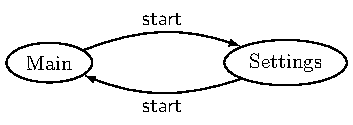
\includegraphics[width=1.9in]{act-running-example1.pdf}
            \label{fig:cmp-atg}
        \end{minipage}
        }
        \subfigure[\cite{LHR17}] {
        \begin{minipage}[t]{0.31\linewidth}
            \centering
            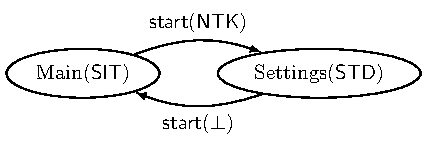
\includegraphics[width=1.9in]{act-running-example2.pdf}
            \label{fig:cmp-lhr}
        \end{minipage}
        }
        \subfigure[AMASS] {
        \begin{minipage}[t]{0.31\linewidth}
            \centering
            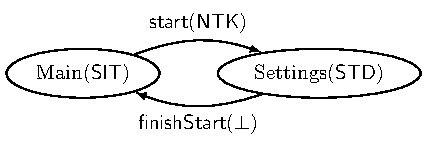
\includegraphics[width=1.9in]{act-running-example3.pdf}
            \label{fig:cmp-amass}
        \end{minipage}
        }
        \caption{Different models for the app LaunchTime Homescreen }
        \label{fig:cmp-models}
    \end{figure}

In the sequel, we consider the task unboundedness problem of these models, that is deciding whether the number of activities in some task will be unbounded. 
\begin{itemize}
	\item In ATG, MainActivity and SettingsActivity will be in a task, MainActivity (resp. SettingsActivity) will be pushed into task by the lower (resp. upper) edge. Therefore there exists a task is unbounded in ATG.
	\item In the model of \cite{LHR17}, MainActivity and SettingsActivity will be placed in two different tasks, since the launch mode of  MainActivity is singleInstance, the number of MainActivity is at most 1. However each time the upper edge is called, SettingsActivity will be pushed into a task, leading to the task unboundedness.
	\item In AMASS, we assume that the label of lower edge is $\startactivity(\bot)$ first, since the real activity of the task containing SettingsActivity is SettingsActivity, SettingsActivity will not be pushed into the task which contains SettingsActivity when the upper edge is called. Therefore, even though finish() function is ignored in AMASS, the task of SettingsActivitys is still bounded. If we do not consider the real activity, only consider the finish() function, the task of SettingsActivitys is still bounded, since when the lower edge is called, SettingsActivity will be finished.
\end{itemize}
Therefore, we can see that ATG and the model of \cite{LHR17} will report the task unboundedness when analyzing the app LaunchTime Homescreen, but either the number of MainActivity or SettingsActivity will be bounded when the app LaunchTime Homescreen is running.
}
%%%%%%%%%%%%%%%%%%%%%%%%%%%%%
%%%%%%%%%%%%%%%%%%%%%%%%%%%%%

%
\revision{\subsection{The ``ShoppingList'' app: fragment-container unboundedness}}
If a model of Android multitasking mechanism does not capture the fragments, then the fragment-container unboundedness problem will be missed in the static analysis of Android apps. 
Furthermore, if the fragments are captured, but in an imprecise way, then the static analysis may still be inaccurate. Let us use the ``ShoppingList'' app to illustrate this point. 
The ``ShoppingList'' app comprises two activities, MainActivity and SettingsActivity. The MainActivity contains five Fragments. Let us focus on three of them, namely, ErrorFragment, ShoppingListFragment and CacheListFragment. From the snippet of the source code in Figure~\ref{code-shoplist}, ErrorFragment can start ShoppingListFragment and CacheListFragment via replace() function (see line 69 and 75 of the ErrorFragment.java file). On the other hand, ShoppingListFragment can start ErrorFragment via replace() function (see line 392 of the ShoppingListFragment file). 
%
\begin{itemize}
\item If an imprecise model for fragments, e.g. the AFTG model in \cite{CHGD18}, is used, then we may wrongly reports that ``ShoppingList'' app suffers from the fragment-container unboundedness problem. The AFTG model extends the ATG model by taking the fragments into consideration and consider all the transitions between them. Nevertheless, the AFTG model does not distinguish between the add and replace actions. As a result, from the existence of a cycle between ErrorFragment and ShoppingListFragment in the AFTG model, we may report that the ``ShoppingList'' app is fragment-container unbounded. 
%
\item On the other hand, if the {\AMASS} model is used, then we can add labels to the edges in the AFTG model and distinguish between the add and replace actions. Then we know that the two edges between ErrorFragment and ShoppingListFragment are both labeled by the replace action. As a result, before ErrorFragment or ShoppingListFragment is pushed to the fragment container, the fragment container is emptied. We conclude that the cycle between ErrorFragment or ShoppingListFragment does not lead to the fragment-container unboundedness problem. 
\end{itemize}
This example motivates us to capture the information about fragments, in particular, distinguish between different fragment actions, in the definition of the {\AMASS} model.

%%%%%%% removed %%%%%%%%%
%%%%%%% removed %%%%%%%%%
\hide{
Figure~\ref{fig:cmp-models-frg} shows two models for the app ShoppingList, Figure~\ref{fig:cmp-aftg} is AFTG and Figure~\ref{fig:cmp-amass-frg} is AMASS. 
In these two models, the Error, ShoppingList and CacheList states represent the ErrorFragment, ShoppingListFragment and CacheListFragment respectively, the edges represent the relation between fragments. Moreover the label $\REP$ of the edge in Figure~\ref{fig:cmp-amass-frg} represents the function replace(). 
AFTG only considers the relation between fragments, ignores the function replace(). In the sequel, we consider the fragment stack unboundedness problem of AFTG and AMASS, that is deciding whether the number of fragments in some fragment stack will be unbounded.
\begin{itemize}
	\item In AFTG, ErrorFragment (resp. ShoppingListFragment) will be pushed into the fragment stack by the edge (ShoppingList, Error) (resp. (Error, ShoppingList)). Therefore the fragment stack is unbounded.
	\item In AMASS, when starting ErrorFragment (resp. ShoppingListFragment) by the edge (ShoppingList, $\REP$, Error) (resp. (Error, $\REP$, ShoppingList)), the fragment stack will be cleared first, hence the number of fragments will be only 1.
\end{itemize}
Therefore, we can see that AFTG will report the fragment stack unboundedness when analyzing the app ShoppingList, but AMASS will not.
}
%%%%%%% removed %%%%%%%%%
%%%%%%% removed %%%%%%%%%

\begin{figure}[htbp]
    \centering
    \begin{tabular*}{\linewidth}{l}
    \begin{lstlisting}
    // app/src/main/java/org/janb/shoppinglist/fragments/ErrorFragment.java 
    63      public void onClick(View view) {
    64          android.app.FragmentManager fragmentManager = getFragmentManager();
    65          FragmentTransaction transaction = fragmentManager.beginTransaction();
    66          switch (view.getId()) {
    67              case R.id.error_btn_retry:
    68                  ShoppingListFragment listFR = new ShoppingListFragment();
    69                  transaction.replace(R.id.fragment_container, listFR);
    70                  transaction.addToBackStack(null);
    71                  transaction.commit();
    72                  break;
    73              case R.id.error_btn_cache:
    74                  CacheListFragment cacheFR = new CacheListFragment();
    75                  transaction.replace(R.id.fragment_container, cacheFR, "CACHE_FRAGMENT");
    76                  transaction.addToBackStack(null);
    77                  transaction.commit();
    78                  break;
                    ...
    83          }
    84      }
    // app/src/main/java/org/janb/shoppinglist/fragments/ShoppingListFragment.java 
    378     public void onError(ResponseHelper error) {
                ...
    385         ErrorFragment errFR;
                ...
    390         FragmentManager fragmentManager = getFragmentManager();
    391         FragmentTransaction transaction = fragmentManager.beginTransaction();
    392         transaction.replace(R.id.fragment_container, errFR);
    393         transaction.addToBackStack(null);
    394         transaction.commitAllowingStateLoss();
    395     }

    \end{lstlisting}
    \end{tabular*}
    \caption{Source code of the F-Droid app ``ShoppingList''}
    \label{code-shoplist}
    \end{figure}


%%%%%%%%%%%%%
%%%%%%%%%%%%%
\hide{
    \begin{figure}[htbp]
        \subfigure[AFTG] {
        \begin{minipage}[t]{0.47\linewidth}
            \centering
            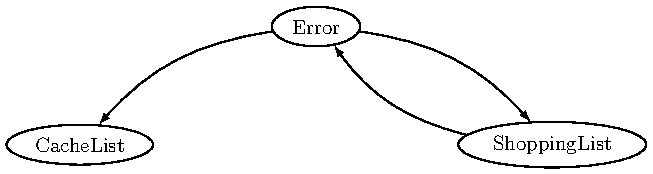
\includegraphics[width=2.5in]{frag-running-example1.pdf}
            \label{fig:cmp-aftg}
        \end{minipage}
        }
        \subfigure[AMASS] {
        \begin{minipage}[t]{0.47\linewidth}
            \centering
            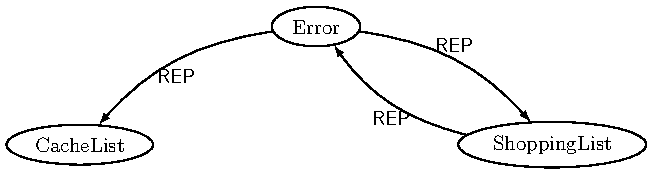
\includegraphics[width=2.5in]{frag-running-example2.pdf}
            \label{fig:cmp-amass-frg}
        \end{minipage}
        }
        \caption{Different models for the app ShoppingList }
        \label{fig:cmp-models-frg}
    \end{figure}
}